\section{TOCL+ Tool Support and Implementation}

\hspace{1cm} Figure \ref{sec:plugin_support_tool_architecture} illustrates the 
architecture and workflow of our TOCL+ support tool. This integrated verification 
framework combines several components: the existing USE environment, the Filmstrip 
plugin, our TOCL+ plugin, and the Model Validator. The architecture maintains a 
clear separation between modeling, specification, and verification concerns while 
providing a cohesive workflow for users.

The verification process consists of five distinct steps, beginning with preparation 
and ending with validation. First, the user prepares two input files: a standard 
\texttt{.use} file containing the UML/OCL application model and a \texttt{.tocl} 
file containing TOCL+ property specifications. Second, the user loads the application 
model into USE to make it available for transformation. Third, the user activates 
our plugin through the USE interface, selecting both a destination path for the 
output model and the \texttt{.tocl} file containing the temporal properties to verify.

Internally, the plugin then executes a two-phase transformation process. In the 
first phase, it invokes the Filmstrip plugin to transform the application model 
into a filmstrip model following the rules described in Section~\ref{subsec:filmstripping}. 
In the second phase, it processes the TOCL+ expressions using our ANTLR4-generated 
parser and listener components, which implement the transformation rules for 
converting temporal specifications into equivalent OCL constraints. These generated 
constraints are added to the list of invariants in the output model file alongside 
the filmstrip model elements.

Finally, the user loads the output model into USE with a configuration file setting search bounds, then uses the Model Validator to analyze the constraints. The validator explores the search space to determine property satisfaction and provides model instances as evidence when applicable.
% To complete the verification process, the user loads this output model back into 
% USE together with a configuration file that establishes search bounds, and then 
% employs the Model Validator to analyze the constraints. The validator systematically 
% explores the search space, determining whether the temporal properties are satisfied 
% and providing a model instance as evidence when applicable.

\begin{figure}[H]
    \centering
    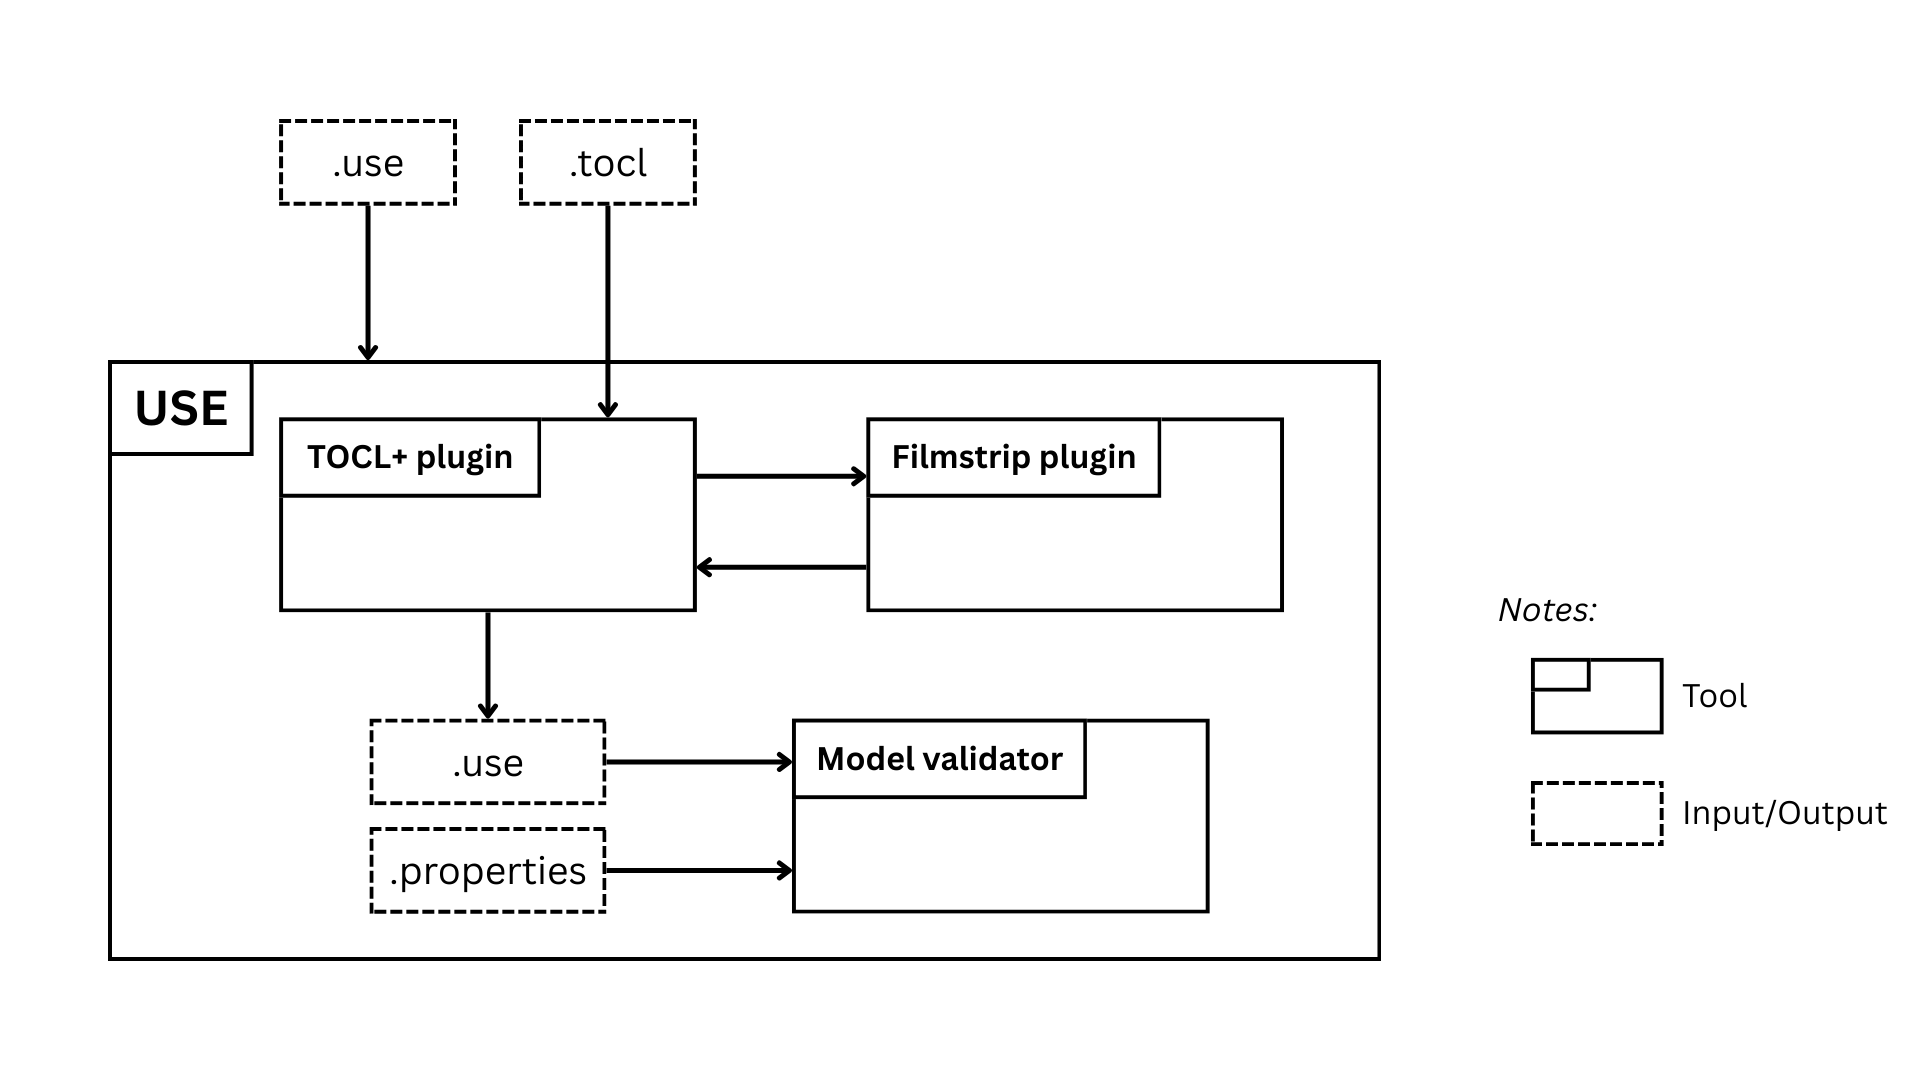
\includegraphics[width=1\textwidth]{figures/c3/Architecture_overview.png}
    \caption{Support Tool Architecture and Verification Workflow.}
    \label{sec:plugin_support_tool_architecture}
\end{figure}

Our primary contribution in this architecture is the TOCL+ plugin, specifically 
the TOCL+ to OCL transformation component that enables the verification of temporal 
properties using existing OCL tools. The implementation details of this transformation 
process, including the translation rules for different temporal operators and event 
constructs, were presented previously in Section \ref{sec:translation}. Our implementation 
follows the transformation patterns established in Chapter 2 and integrates them into 
the workflow described above.

% Our primary contribution in this architecture is the TOCL+ plugin, specifically 
% the TOCL+ to OCL transformation component that enables the verification of temporal 
% properties using existing OCL tools. The implementation details of this transformation 
% process, including the translation rules for different temporal operators and event 
% constructs, are presented in the next subsection.

% \subsection{Implementation of TOCL+ to OCL Transformation}

% \hspace{1cm} The core of our contribution lies in the transformation of TOCL+ 
% expressions into equivalent OCL constraints that can be verified over filmstrip 
% models. This transformation process involves systematically mapping temporal operators 
% and event constructs to structural navigations through snapshots and operation calls. 
% In this section, we describe our implementation approach and the key translation 
% patterns we developed.

% Our transformation approach is inspired by the work of \cite{TOCL2OCL}, who 
% transformed TOCL \cite{TOCL} into OCL in the context of a Snapshot-Transition Model 
% (STM). While their approach also converts temporal properties into static ones, we 
% adapted and extended it to work within the filmstrip model context.

% To transform TOCL+ expressions, we defined translations for TOCL+ operators and 
% events to OCL, as shown in Table \ref{tab:TOCL2OCL}. To create these translations, 
% we utilized several query operations provided by the filmstrip structure. 
% The self.snapshot query accesses the snapshot associated with an object in the 
% "current state" where the expression is being evaluated. The pred() and succ() 
% operations, when applied to a snapshot, navigate to the previous and next state 
% respectively. For objects to navigate to their corresponding versions in adjacent 
% states, we use the two associations .pred and .succ. These navigation mechanisms 
% form the foundation for implementing our temporal operator translations.

% Note that filmstrip model does not inherently provide any means to identify the same 
% logical object across different states - it only provides the .pred and .succ 
% associations to navigate between corresponding objects in adjacent snapshots. 
% In order to overcome this limitation, we require modelers to add an id attribute 
% to all classes in the application model. As seen in Figure \ref{fig:object_diagram_liveness}, 
% this allows us to identify the same logical object across different snapshots. 
% Internally, when the TOCL+ plugin transforms the model, we add additional 
% constraints to ensure this id remains consistent between different states. 
% This id attribute is critical in the OCL translation, particularly for event 
% constructs like becomesTrue. When navigating with expressions like 
% self.snapshot.pred().[ContextObject], we get a collection of objects of the same 
% type, and we select the one with matching identity using ->any(o | o.id = self.id).

% Table \ref{tab:TOCL2OCL} presents the complete set of translation patterns we 
% developed for TOCL+ operators and event constructs. Each pattern systematically 
% maps a TOCL+ construct to an equivalent OCL expression interpreted over the filmstrip 
% model. The patterns use placeholders (indicated by square brackets) that get 
% substituted during the transformation process: \texttt{[s |= P]} indicates that 
% property P holds in snapshot s; \texttt{[ContextSnapshot]} is the snapshot in which 
% the property is evaluated; \texttt{[ContextObject]} is the object on which the 
% property is evaluated; \texttt{[OpClassName]} is the class representing an 
% operation call in the filmstrip model; and \texttt{[ContextClass]} is the class name
% representing the context of the current evaluation. When applying these patterns, 
% each placeholder is replaced with the appropriate expression based on the model 
% context. For example, in the liveness property translation shown in Listing 
% \ref{lst:ocl_liveness}, the \texttt{[ContextSnapshot]} is replaced with the local variable 
% \texttt{s} inside the \texttt{exists} query; the bounded quantifiers (e.g., \texttt{at most}, 
% \texttt{at least}) are translated into corresponding comparators (\texttt{<=}, \texttt{>=}). 
% The bounded quantifiers in TOCL+ expressions are systematically translated into their 
% corresponding OCL comparators: \texttt{at most} becomes less than or equal to 
% (\texttt{<=}), while \texttt{at least} becomes greater than or equal to (\texttt{>=}). 
% For bounded existence properties without an explicit quantifier (e.g., 
% \texttt{isCalled(Op()) 3 times}), the translation applies the equality operator 
% (\texttt{=}), enforcing that the event occurs exactly the specified number of times. 
% In contrast, when dealing with unbounded event expressions without quantifiers (e.g., 
% simply \texttt{isCalled(Op())}), the translation converts the \texttt{select} operation 
% into an \texttt{exists} operation, requiring only that the event occurs at least once 
% rather than counting occurrences.
    
% We implemented the transformation using ANTLR4, a parser generator that creates a 
% parse tree from TOCL+ expressions. After defining the translation patterns shown 
% in Table \ref{tab:TOCL2OCL}, we created Java listener classes that extend the 
% generated parser listeners. The transformation process employs these listener 
% components to traverse the parse tree and produce corresponding OCL expressions 
% by overriding the generated listener methods. As the parser walks through each node 
% in the parse tree, our listeners intercept parse tree events and apply the appropriate 
% translation rules, constructing equivalent OCL constraints that navigate through 
% the filmstrip structure. The transformation follows a consistent pattern: when a 
% temporal operator or event construct is encountered, the listener extracts relevant 
% information from the parse tree nodes, applies the corresponding translation pattern, 
% and builds the equivalent OCL expression. Our implementation maintains a stack of 
% expressions to handle nested structures, pushing both the original TOCL+ expression 
% and its OCL translation for later integration into the output model.
% Listing \ref{lst:becomesTrue_translation} provides an example of this process for 
% the \texttt{becomesTrue} event construct, showing how we extract the expression 
% to be evaluated, establish the necessary context, and construct the translated OCL 
% expression. 

% After processing all the nodes in the parse tree, our implementation finalizes the 
% translation in the root node visit. Since TOCL+ is an extension of OCL, many 
% constructs remain unchanged and are directly preserved during translation. The 
% completion process begins by accessing the token stream to retrieve the complete 
% original expression text. Our implementation then systematically pops each translated 
% OCL fragment and its corresponding original TOCL+ expression from the stack. Using 
% string replacement operations, it substitutes each temporal construct with its 
% equivalent OCL translation while preserving the structure of the original expression. 
% This approach allows us to handle nested temporal operators naturally, as inner 
% expressions are processed before their containing expressions. The final translated 
% OCL constraint is then attached to the root of the parse tree and ultimately added 
% to the output model as an invariant. This complete process ensures that complex 
% temporal properties are accurately transformed into standard OCL constraints that 
% can be verified by the Model Validator.

% \begin{lstlisting}[
%     style=javastyle,
%     caption={Translation of becomesTrue event to OCL.},
%     label={lst:becomesTrue_translation}
% ]
% TokenStream tokens = parser.getTokenStream();
% String originalEvent = tokens.getText(ctx);
% String translatedEvent;
% // P
% String expressionToSatisfy = getOCL(ctx.getChild(2)); 
% // e.g., "system", "application"
% String roleName = toLowerFirstChar(currentContext); 
% String currentSnapshot = "self.snapshot"; 
% String selectObject = "->any(o | o.id = self.id)";

% // e.g. self.snapshot.system->any(o | o.id = self.id)
% String objectAtCurrentSnapshot = currentSnapshot + "." + roleName + selectObject;
% String objectAtPreviousSnapshot = currentSnapshot + ".pred()." + roleName + selectObject;
% String P_at_currentSnapshot = expressionToSatisfy.replace("self", "currentObject");
% String P_at_previousSnapshot = expressionToSatisfy.replace("self", "previousObject");

% translatedEvent = 
% "let currentObject = " + objectAtCurrentSnapshot +
% " in let previousObject = " + objectAtPreviousSnapshot +
% " in not (" + P_at_previousSnapshot + ") and (" + P_at_currentSnapshot + ")";

% eventStack.push(translatedEvent);
% eventStack.push(originalEvent);    
% \end{lstlisting}

% \begin{longtable}{|>{\footnotesize}p{0.6cm}|>{\scriptsize\raggedright\arraybackslash}p{4cm}|>{\scriptsize\raggedright\arraybackslash}p{\dimexpr\textwidth-4.6cm-4\tabcolsep-3\arrayrulewidth\relax}|}
%     \caption{Translation of TOCL+ operators and events to OCL.}
%     \label{tab:TOCL2OCL} \\
%     \hline
%     \textbf{No.} & \textbf{TOCL+} & \textbf{OCL Translation} \\
%     \hline
%     1 & 
%     next P &
%     let nextSnapshot:Snapshot = self.snapshot[ContextClass].succ() in [nextSnapshot |= P] \\
%     \hline
%     2 &
%     always P &
%     let CS:Snapshot = self.snapshot[ContextClass] in Set\{CS\}->closure(s | s.succ())->forAll(s | [s |= P]) \\
%     \hline  
%     3 &
%     always P until Q &
%     let CS:Snapshot = self.snapshot[ContextClass]
%     in let FS:Set(Snapshot) = Set\{CS.succ()\}->closure(s | s.succ())
%     in let AllFSQ:Set(Snapshot) = FS->select(s | [s |= Q])
%     in let FSQ:Snapshot = AllFSQ->any(s | Set\{s\}->closure(s | s.succ())->includesAll(AllFSQ))
%     in let afterQ:Set(Snapshot) = Set\{FSQ\}->closure(s | s.succ())
%     in let FSP:Set(Snapshot) = FS->select(s | [s |= P])
%     in if FSQ.isDefined() then (if (FSP->size() > 0) then (FS-afterQ = FSP-afterQ) else false endif) else (FS = FSP) endif \\
%     \hline
%     4 &
%     always P since Q &
%     let CS:Snapshot = self.snapshot[ContextClass]
%     in let PS:Set(Snapshot) = Set\{CS.pred()\}->closure(s | s.pred())
%     in let AllPSQ:Set(Snapshot) = PS->select(s | [s |= Q])
%     in let PSQ:Snapshot = AllPSQ->any(s | Set\{s\}->closure(s | s.pred())->includesAll(AllPSQ))
%     in let beforeQ:Set(Snapshot) = Set\{PSQ\}->closure(s | s.pred())
%     in let PSP:Set(Snapshot) = PS->including(CS)->select(s | [s |= P])
%     in if PSQ.isDefined() then (if (PSP->size() > 0) then (PS->including(CS)-beforeQ = PSP-beforeQ) else false endif) else (PSP = PS->including(CS)) endif \\
%     \hline
%     5 &
%     sometime P &
%     let CS:Snapshot = self.snapshot[ContextClass] in Set\{CS\}->closure(s | s.succ())->exists(s | [s |= P]) \\
%     \hline
%     6 &
%     sometime P before Q &
%     let FS:Set(Snapshot) = Set\{self.snapshot[ContextClass]\}->closure(s | s.succ())
%     in let PreS:Set(Snapshot) = Set\{self.snapshot[ContextClass].pred()\}->closure(s | s.pred())
%     in let AllFSQ:Set(Snapshot) = FS->select(s | [s |= Q])
%     in let FSQ:Snapshot = AllFSQ->any(s | Set\{s\}->closure(s | s.succ())->includesAll(AllFSQ))
%     in let FSP:Set(Snapshot) = FS->select(s | [s |= P])
%     in if FSQ.isDefined() then (if (FSP->size() > 0) then ((Set\{FSQ.pred()\}->closure(s | s.pred())-PreS)->exists(s\_1 | FSP->includes(s\_1))) else false endif) else false endif \\
%     \hline
%     7 &
%     sometime P since Q &
%     let CS:Snapshot = self.snapshot[ContextClass]
%     in let PS:Set(Snapshot) = Set\{CS.pred()\}->closure(s | s.pred())
%     in let AllPSQ:Set(Snapshot) = PS->select(s | [s |= Q])
%     in let PSQ:Snapshot = AllPSQ->any(s | Set\{s\}->closure(s | s.pred())->includesAll(AllPSQ))
%     in let PSP:Set(Snapshot) = PS->select(s | [s |= P])
%     in if PSQ.isDefined() then (Set{PSQ}->closure(s | s.succ())->excluding(null)->intersection(PS)->exists(s | PSP->includes(s))) else false endif \\ 
%     \hline
%     8 &
%     previous P &
%     let previousSnapshot:Snapshot = self.snapshot[ContextClass].pred() in [previousSnapshot |= P] \\
%     \hline
%     9 &
%     sometimePast P &
%     let CS:Snapshot = self.snapshot[ContextClass] in Set\{CS.pred()\}->closure(s | s.pred())->exists(s | [s |= P]) \\
%     \hline
%     10 &
%     alwaysPast P &
%     let CS:Snapshot = self.snapshot[ContextClass] in Set\{CS.pred()\}->closure(s | s.pred())->forAll(s | [s |= P]) \\
%     \hline
%     11 &
%     isCalled(Op()) &
%     [OpClassName].allInstances()->exists(op | op.succ() = [ContextSnapshot]) \\
%     \hline
%     12 &
%     isCalled(Op($param_1$, $\ldots$, $param_n$)) &
%     [OpClassName].allInstances()->exists(op | op.succ() = [ContextSnapshot] and
%     (Set\{op.$param_1$.succ\}->closure(p | p.succ)->includes($param_1$) or Set\{op.$param_1$.pred\}->closure(p | p.pred)->includes($param_1$))
%     and ($\ldots$)
%     and (Set\{op.$param_n$.succ\}->closure(p | p.succ)->includes($param_n$) or Set\{op.$param_n$.pred\}->closure(p | p.pred)->includes($param_n$))) \\
%     \hline
%     13 &
%     isCalled(Op()) [at most | at least | ] n times &
%     [OpClassName].allInstances()->select(op | op.succ() = [ContextSnapshot])->size() [<= | >= | =] n \\
%     \hline
%     14 &
%     isCalled(Op($param_1$, $\ldots$, $param_n$)) [at most | at least | ] n times &
%     [OpClassName].allInstances()->select(op | op.succ() = [ContextSnapshot] and
%     (Set\{op.$param_1$.succ\}->closure(p | p.succ)->includes($param_1$) or Set\{op.$param_1$.pred\}->closure(p | p.pred)->includes($param_1$)) 
%     and ($\ldots$) 
%     and (Set\{op.$param_n$.succ\}->closure(p | p.succ)->includes($param_n$) or Set\{op.$param_n$.pred\}->closure(p | p.pred)->includes($param_n$)))->size() [<= | >= | =] n \\
%     \hline
%     15 &
%     becomesTrue(P) &
%     let currentObject = self.snapshot[ContextClass].[ContextObject]->any(o | o.id = self.id) in
%     let previousObject = self.snapshot[ContextClass].pred().[ContextObject]->any(o | o.id = self.id) in 
%     not [previousObject |= P] and [currentObject |= P] \\
%     \hline
% \end{longtable}
